\chapter{Estudio del Problema Singular}
{\label{cap.singular}}

El presente capítulo contiene el resultado original de este Trabajo de Diploma, que consiste en el análisis de un operador diferencial con un coeficiente singular. Como hemos mencionado, el desarrollo asintótico (\ref{eq.heat.expansion})
es válido para operadores diferenciales con coeficientes suaves. En efecto,
mostraremos a continuación que la presencia de una singularidad puede
conducir a un desarrollo asintótico de la traza del heat-kernel que no con-
tiene exclusivamente potencias semi-enteras de t. Veremos que
en el caso del operador singular que hemos analizado el desarrollo contiene
términos $\log t$.

Aquí se van aplicar las herramientas desarrolladas en el capitulo anterior
al estudio del espectro de un operador singular en un intervalo compacto,
encontrando una contradicción al teorema (\ref{eq.heat.expansion}), a su vez se va a generar un scipt de Mathematica que permite graficar distintas aproximaciones a
la parte finita de la energía de vacío.


\section{El Operador Singular}


En está sección se estudiará el siguiente operador diferencial definido sobre funciones en el intervalo $[0,L]$,
\begin{equation}
\begin{aligned}
    A \phi (x) &= - \partial ^2 _x  \phi(x) + \frac{\alpha}{x} \phi(x) \\[5pt]
    \phi(0) &= \phi(L) = 0 \, .
\end{aligned}
\label{operador}
\end{equation}
Por simplicidad, imponemos condiciones Dirichlet en ambos extremos. El parámetro $\alpha \in \mathbb{R _{+}}$ caracteriza la singularidad en el origen.

Los autovalores están dados por la ecuación 
\begin{equation}
\begin{aligned}
    A  \phi (x)  &=   \lambda ^2 \phi (x) \\[5pt]
    \lambda ^2 \ &\in \ \mathbb{R}  
    \, ,
\end{aligned}
\label{eq.aut.sin}
\end{equation}
Las autofunciones, en términos de dos soluciones linealmente independientes $\phi _1 (x), \phi _2 (x)$ de (\ref{eq.aut.sin}), pueden escribirse
\begin{equation}
\begin{aligned}
    \phi (x) =
	    C _1
    	\underbrace{
				     \ e ^{-i \lambda x} \ x \ 
				     F _{1} ^{1} 
				     		\left(  
				     			1 - \frac{i \alpha}
				     			{2\lambda}
				     		,2,2 i \lambda x \right) 
				     } _ {\phi_1} + 
      C _2 
      \underbrace{ 
      			   \ e^{-i \lambda x } \ x \ 
      			   U 
      			   	\left( 
      			   		1- \frac{i \alpha}{2 \lambda}
      			   		,2,2 i \lambda x \right) } _{\phi_2} 
    \, . 
\end{aligned}
\label{eq.phi}
\end{equation}
Donde $F _1 ^1(a,b,z)$ y $ U(a,b,z)$ son las soluciones LI de la ecuación hypergeométrica
\begin{equation}
    z \ \partial ^2 _z \ \psi (a,b,z) + (b-z) \
    \partial _z \psi (a,b,z)
    -a \ \psi (a,b,z) = 0 \, .
\end{equation}
las cuales están dadas por \cite{Abramowitz:hyper}
\begin{align}
	U(a,b,z) = &\frac{1}{\Gamma (a)} 
	\int _0 ^{\infty} e ^{-zt}
	t ^{a-1}
	(1+t) ^{b-a-1}
	dt \\
	& {\rm si \ } Re (b) > Re(a) 
	\nonumber
	\\[5pt]
	F _1 ^1 (a,b,z) =& \sum _ {k=0} ^{\infty} 
	\frac{(a) _k}{(b) _k} 
	\frac{z ^k}{k!} 
	\, ,
\end{align}
donde $(.) _n$ es el símbolo de Pochhammer.
Si se cumple que  $a=-m,b \neq -n$ donde $ m,n \in \mathbb{N}$, $F _1 ^1 (a,b,z)$ es un polinomio en $z$ y $U(a,b,z)$ es linealmente dependiente con $F _1 ^1 (a,b,z)$, en tal caso se usa $z^{1-b} M(a+1,-b,2-b,z)$ como segunda solución LI.


Las constantes $C_1,C_2$ están sujetas al vínculo impuesto por las condiciones de contorno.
Para imponer las condiciones de contorno, primeramente desarrollamos $\phi (x)$ cerca de $x \simeq 0$ 
\begin{align}
\phi  ( x ) &=
C _1  x  + 
C _2 \ x 
\left( 
\frac{1}{  \alpha x  \Gamma ( - \frac{i \alpha}{2  \lambda}  )   }  +
\frac{\log (x) }{\Gamma ( - \frac{ i \alpha}{2 \lambda} ) } + \mathscr{C} \right) + O(x ^2)
	\nonumber
\\[10pt]
\mathscr{C} &= 
\frac{
-1 + 2 \gamma + \log ( 2  i \lambda ) + \psi (1 - \frac{i \alpha}{2 \lambda})
}
{\Gamma (\frac{i \alpha}{2 \lambda})}
\, ,
\label{eq.scat}
\end{align}
de este desarrollo se ve que $ \phi _1 (x \rightarrow 0 ) \rightarrow 0,\phi _2 (x \rightarrow 0)  \rightarrow
\frac{1}{  \alpha   \Gamma ( \frac{i \alpha}{2 \lambda}  )   } $ , entonces la condición de contorno en $x=0$ fija $C _2 =0$. En caso de que $\Gamma ( \frac{i \alpha}{2 \lambda}  ) \rightarrow \infty$, $\phi _2 (0) = 0$.


Utilizando la condición de contorno en $x=L$ los autovalores están dados por las soluciones de la siguiente ecuación
\begin{equation}
F _1 ^1 \left(1-\frac{i \alpha}{2 \lambda},2,2 i \lambda L \right)  = 0
	\, .
\label{eq.1}
\end{equation}
En la figura (\ref{fig:funcion}) graficamos
\mbox{$ | F _1 ^1 (1-\frac{i \alpha}{2 \lambda},2,2 i \lambda L) | ^2 $} para los valores  $\alpha=1, \ L=1$. Las intersecciones con el eje horizontal indican los autovalores positivos del espectro del operador singular.

\begin{figure}[h!]
\centering
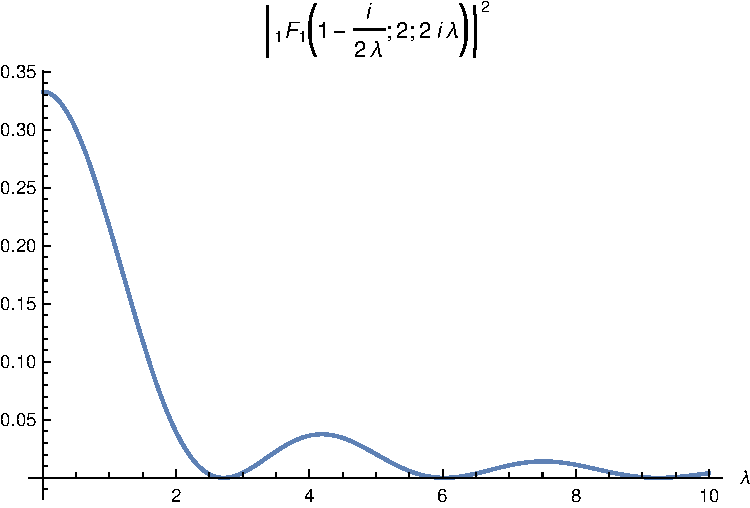
\includegraphics[scale=0.7]{Funcion.pdf}
\caption{En esta imagen se puede ven ver los primeros ceros de la función $| F _1 ^1 (1+\frac{ \alpha}{2 i \lambda},2,2 i \lambda L) | ^2$, para $\alpha=1$ y $L=1$, los cuales representan a los primeros autovalores de $A$.}
\label{fig:funcion}
\end{figure}

Más adelante utilizaremos el desarrollo asintótico de la funcion $F _1 ^1 (a,b,z)$ para $z \rightarrow \infty$, \cite{Abramowitz:hyper},
\begin{equation}
\begin{aligned}
    F _1 ^1 (a,b,z) &= \Gamma (b) 
    \left(
    \frac{e^z z ^{a-b} }{\Gamma(a)}  S_1 (z) + \frac{(-z) ^{ -a}}{ \Gamma(b-a)} 
    S_2 (z)
    \right) \\[5pt]
    S _1 (z) &= \sum _{n=0} ^{\infty} \frac{(b-a) _n (1-a) _n}{n!} z ^{-n} \\[5pt]
    S _2 (z) &= \sum _{n=0} ^{\infty} \frac{(a) _n (1+a-b) _n}{n!} (-z) ^{-n}     
		\, .
\end{aligned}
\label{eq.aprox}
\end{equation}
$S_1$ y $S _2$ representan el desarrollo a todo orden. Para calcular el polo de la {\it función-$\zeta$} en $s=-1/2$ basta tomar $S _1 = S _2 = 1$ que es lo que se hará a continuación, para conocer los polos mas hallá de $s=-1/2$ o para estudiar la parte finita de $\zeta (-1/2)$ se deben tomar mas términos en $S_1$ y $S _2$, lo cual se hará al final de este capítulo en las secciones \ref{sec.sig.polos} y \ref{sec.regular}.


Utilizando (\ref{eq.aprox}) y tomando $S _1 = S _2 = 1$, $F _1 ^1 \left(1+  \frac{  \alpha}{2 i \lambda} ,2 ,2 i \lambda L  \right)$ está dado por
\begin{equation}
    \frac{i e ^{ \frac{\pi \alpha }{4 \lambda}  } }{2 \lambda L}
    \left(
    \frac{e ^{   \frac{ i \alpha}{2 \lambda}  \log (2 \lambda L) }}               {\Gamma(1+\frac{i \alpha}{2 \lambda})} -
    \frac{e ^{-  \frac{i \alpha}{2 \lambda}  \log (2 \lambda L) } e ^{2 i \lambda L} }{\Gamma(1-\frac{i \alpha}{2 \lambda})} 
    \right) \\[5pt]  
    =  i  \frac{e ^{ \frac{\pi \alpha }{4 \lambda}  } }{2 \lambda L}     M (\lambda) 
    \, ,
\label{eq.completa}
\end{equation}
dado que $M( \lambda)$ posee los mismos ceros que (\ref{eq.completa}), se puede utilizar $M( \lambda)$  para estudiar los polos de la {\it función-$\zeta$} para $s \geq - \frac{1}{2}$, así  como cualquier otra función que contenga los mismos ceros.

\section{Calculo Asintótico de los autovalores}\label{seq.2.asin}

En está sección seguiremos el procedimiento descrito en \ref{seq.asin} para estudiar la estructura de polos de la función $\zeta$: calcularemos el desarrollo asintótico de grandes autovalores, que luego será utilizado para determinar los residuos en los primeros polos $s= \frac{1}{2}$ y $s= - \frac{1}{2}$.



Es conveniente definir las variables adimensionales: $\mu _n = \lambda _nL $ y $\beta = \alpha L$. Luego en vez de utilizar $M (\mu _n)$ definida en (\ref{eq.completa}) se trabajará una función $N (\mu _n)$ que posee los mismos ceros, definida de la forma
\begin{align}
\nonumber
N (\mu _n) &=
e ^{\frac{i \beta }{\mu _n} \log(2 \mu _n) }
\Gamma \left( 1 + \frac{ \beta}{2 i \mu _n} \right)
M (\mu _n) \\ 
&=  
e ^{\frac{i \beta }{\mu _n} \log(2 \mu _n) }
\frac{\Gamma \left(1 + \frac{ \beta}{2 i \mu _n} \right)}
	{\Gamma \left(1 - \frac{ \beta}{2 i \mu _n} \right)}
- e ^{2 i \mu _n}
\, ,
\label{eq.otro.mu}
\end{align}
en el limite de $\mu _n \rightarrow \infty$ se obtiene
\begin{equation}
    N(\mu _n  \rightarrow \infty) = 
	1 - e ^{2 i \mu _n}
		\, ,
\end{equation}
de aquí puede verse el comportamiento dominante  de $\mu _n$ para grandes valores de $n$
\begin{equation}
\begin{aligned}
    &\mu _n = n \pi + \epsilon _n \\[5pt]
	&\lim \limits _{n \rightarrow{0}} \epsilon _n  = 0
		\, .
\end{aligned}
\label{eq.mu2}
\end{equation}
Reemplazando (\ref{eq.mu2}) en (\ref{eq.otro.mu}), e igualando $N (\mu _n) = 0$ se que $\mu _n$ cumple la ecuación
\begin{equation}
	e ^{ i \frac{\beta}{ \mu _n} \log (2 \mu _n)}     
    \frac{\Gamma(1 + \frac{ \beta}{2  i \mu _n} ) }
    {\Gamma(1 -  \frac{ \beta}{2  i \mu _n} )} =    
    e ^{2 i \epsilon _n }
    	\, .
\label{eq.a.desarrollar}
\end{equation}
Utilizando que  $ \lim \limits_{\mu _n \rightarrow \infty} \frac{\log (2 \mu _n)}{2 \mu _n } \rightarrow 0$, se puede representar \ref{eq.a.desarrollar} por su desarrollo en serie en los límites $ \mu _n \rightarrow \infty $ y $\epsilon _n \rightarrow 0$,
\begin{equation}
    \left(
    \sum _{p = 0} ^{\infty} \frac{ \left( i \frac{\beta}{ \mu _n } \log(2 \mu _n ) \right) ^p }{p!}
    \right)
    \left(
	\sum _{q = 0} ^{\infty} \frac{a _q}{\mu _n ^q}
	\right)
    =
    \left(
    \sum _{l = 0} ^{\infty} \frac{( 2 i \epsilon _n)^l}{l !}
    \right)
    	\, .
\end{equation}
La corrección a $O ( n ^{-1}) $ de $\epsilon _n$ viene dada por
\begin{equation}
\left( 1 + \frac{i \beta}{ \mu _n} \log ( 2 \mu _n) \right) 
\left(1 + \frac{i  \gamma \beta}{ \mu _n} \right)  =
(1 + 2 i \epsilon _n) \, ,
\end{equation}
resultando el orden dominante $\epsilon _n =  \frac{\beta }{2 n \pi}  \log (2 n \pi)$, lo cual no es suficiente para hallar el polo en $s=- \frac{1}{2}$ ya que existe otro termino que decae como $ n ^{-1}$, reemplazando $\epsilon _n =  \frac{\beta }{2 n \pi} \log (2 n \pi) + \epsilon '$ en la ecuación anterior, se obtiene
\begin{equation}\label{anterior}
    \epsilon _n =  \frac{\beta }{2 n \pi} \log (2 n \pi) +
                \frac{\gamma \beta}{2 n \pi} +
                O\left(  \frac{1}{n^2} \right)
                	\, .
\end{equation}
Para calcular la {\it función-$\zeta $} se utiliza su definición
\begin{equation}
\begin{aligned}
    \zeta (s) &= \sum _{n=1} ^{\infty} \left( \frac{\lambda _n}{\mu} \right) ^{-2 s}  \\
    & =    ( \mu L) ^{2 s} \sum _{n=1} ^{\infty} 
    \left( 
    n \pi + \frac{\alpha L }{2 n \pi} \log (2 n \pi) + \frac{\gamma \alpha L}{2 n \pi} +
    O \left( n^{-2} \right)
    \right) ^{-2s}
    	\, ,
\end{aligned}
\end{equation}
la cual se puede reescribir como
\begin{equation}
\begin{aligned}
    \zeta  (s) &= \left( \frac{\mu L }{\pi} \right)  ^{2 s} 
    \sum _{n=1} ^{\infty} n ^{- 2  s} 
    \left(
    	1 + \chi _n  + O( n^{-2} )
    	\right) ^{-2 s} \\[5pt]
		 \chi _n &= 
    	\frac{\alpha L  }{2 n^2 \pi ^2} \log (2 n \pi) + 
    	\frac{\gamma \alpha L}{2 n^2 \pi ^2 }  
    			\, .
\end{aligned}
\end{equation}
Desarrollando consistentemente hasta el orden retenido se obtiene
\begin{align}\label{eq.zeta.c}
    \zeta  (s) &= \left( \frac{\mu L}{\pi} \right) ^{2 s}
    \sum _{n=1} ^{\infty} 
    n ^{-2s}
    \left(
    1 - 2 s \chi _n + O \left( n ^{-3} \right) \
    \right)   \nonumber \\[5pt]
     &= \left( \frac{\mu L }{\pi} \right) ^{2 s}
    \sum _{n=1} ^{\infty} n ^{-2 s} 
    \left(
    1 - 2s \left(
    \frac{\alpha L }{2 n ^2 \pi ^2} \log ( 2  n \pi) + 
    \frac{\gamma \alpha L }{2 n ^2 \pi ^2} 
	\right) +
    O \left( n ^{-3}   \right)
    \right) \nonumber \\[5pt]
    &=   \left( \frac{\mu L }{ \pi } \right) ^{2 s}  
    \left( \zeta _R (2 s) -
	\frac{ s \alpha L}{ \pi ^2} \zeta _R (2s+2)
	\left(
	    \log (2  \pi ) + \gamma
	\right) + 
    \frac{s \alpha L}{\pi ^2}
	\zeta ' _R(2s+2) \right) \nonumber \\[5pt]
	&\ \ \ \  + \sum _{n=1} ^{\infty} O \left( n ^{-2s-3} \right) \, .
\end{align}    
Donde $\gamma$ es la constante de Euler-Mascheroni.
Dado que $\sum _{n=1} ^{\infty} O \left( n ^{-2s-3} \right)$ es regular para $s > -1$, de la expresión anterior el polo en $s= - \frac{1}{2}$ está dado por
\begin{equation}\label{eq.res.2}
    ( s-1/2 ) \zeta  (s) | _{s \rightarrow \frac{1}{2}} = 
    \frac{\mu L }{2 \pi}
    	\, ,
\end{equation}
lo cual coincide con el resultado general \ref{eq.vol}. Luego desarrollando \ref{eq.zeta.c} alrededor de $s=-1/2$ se obtiene
\begin{align}\label{eq.res.1}
    &\zeta  (s) =  \frac{\alpha}{8  \pi \mu (s+1/2)^2} +
    \frac{ \alpha ( \gamma  +  \log (2\mu L ) -1 ) }{4  \pi \mu (s+1/2) }  + 
	f (s) \\
	&| f(s) | < \infty , \, \forall s > -1
    	\, .
\end{align}
Lo cual muestra el primer resultado de esta tesis, la existencia de un polo doble en $\zeta(-1/2)$ lo cual está en contradicción con (\ref{eq.heat.expansion}).

\section{Cálculo Utilizando Variable Compleja}\label{seq.2.com}


En la sección anterior se estudiaron los polos de la {\it función-$\zeta$} en $s=\frac{1}{2}$ y $s=-\frac{1}{2}$ desarrollando los autovalores.
En esta sección al igual que en la sección \ref{sec.complejo} se va a expresar la {\it función-$\zeta $} como una integral en el plano complejo sin necesidad de conocer los autovalores, obteniendo coincidencia con los resultados (\ref{eq.res.1}) y (\ref{eq.res.2}).

Dado que se van a estudiar los polos en $s=1/2$ y $s=-1/2$ se utilizará la función $M (z)$ definida en (\ref{eq.completa}).
La {\it función-$ \zeta$} queda determinada por
\begin{equation}
\zeta (s) = 
\frac{1}{2 \pi i} 
\int _{\mathcal{C}}
\frac{M ' ( z ) }{ M ( z ) } z ^{-2s} d z = 
\frac{1}{2 \pi i} 
\int _{\mathcal{C}}
\partial _z \ \log 	M(z)  z ^{-2s} \ dz
	\, ,
	\tag{\ref{asd}}
\end{equation}
Se va a utilizar el contorno dado por \ref{fig.derecha}. 
Utilizando la parametrización $ z (t) = \pm i t$ sobre los ejes verticales. El termino $e ^{2 i \lambda L}$ va a generar un termino exponencialmente creciente/decreciente dependiendo de la rama, tirando la parte exponencialmente decreciente en cada rama y la contribución angular, se obtiene para los términos $\log M(z)$ definidos en la ecuación anterior.
\begin{comment}
\begin{equation}
\begin{array}{c}
    \zeta  (s) = \\
     \frac{1}{2 \pi i} \int _{\infty} ^{1}
     \frac{ i \alpha }{2 t^2} 
     \left(
      1 + \frac{i \pi}{2} + Ln[2 t] + \psi (1 + \frac{\beta}{2 t})
     \right)
     t ^{-2s}
     e ^{- i \pi s} (i dt) + \\
     \frac{1}{2 \pi i} \int _{\infty} ^{1} 
     \left(
     2 + \frac{\beta}{2 t^2}
     \left(
     1 + \frac{i \pi}{2} - Ln[2 t] - \psi (1+ \frac{\beta}{2 t})
     \right)
     t ^{-2s}
     e ^{ i \pi s} (-i dt)
     \right)     
\end{array}
\end{equation}
\end{comment}
\begin{align}\label{eq.logatirmos}
\log ( M ( \lambda = i t ) ) &=   
\frac{i \alpha }{2 \lambda}  \log (2 \lambda L) - 
 \log \left( \Gamma \left( 1 - \frac{ \alpha}{2 i \lambda} \right) \right) \\ 
\log ( M ( \lambda=-i t ) ) &=   -  
\frac{i \alpha }{2 \lambda}  \log ( 2 \lambda L ) - 
 \log \left( \Gamma \left( 1 + \frac{ \alpha}{2 i \lambda} \right) \right) +
2 i \lambda L  \nonumber
	\,	,
\end{align}
lo cual conduce a una representación integral de la función $\zeta$ dada por
\begin{align}\label{eq.zeta.logs}
    \zeta  (s) =& \\
     & \frac{e^{-i \pi s} \mu ^{2s}}{2 \pi i} \int _{\infty} ^{1}
     \frac{ i \alpha}{2 t^2}
     \left(
     - 1 +  \log (2 L t) + \frac{i \pi}{2}  - \psi \left( 1+\frac{\alpha}{2 t} \right)
     \right)
     t^{-2 s}
      \nonumber
     (i dt) + \\
     & \frac{e^{i \pi s} \mu ^{2s}}{2 \pi i} \int _1 ^{\infty}
	\left(      
     \frac{ i \alpha}{2  t^2}
     \left(
     1 -  \log (2 L t) + \frac{i \pi}{2} + \psi \left( 1 + \frac{\alpha}{2 t} \right)       
     \right)
     + 2 i L
     \right)
     t^{-2 s}
     (-i dt) \nonumber
     	\, .
\end{align}
El término que tiene la potencia mas alta de $t$ va a contribuir al polo en $s=1/2$, el cual está dado por
\begin{equation}
    \frac{e^{i \pi s} \mu ^{2s} }{2 \pi i }
    \int _1 ^{\infty}
    2 i L    
    t ^{-2 s}
    (-i dt) =  
    \frac{L e^{i \pi s} \mu ^{2s}}{2 \pi i} \frac{1}{s-1/2   }
    	\, ,
\end{equation}
ningún otro término aportará a este polo, entonces coincidiendo con \ref{eq.res.2} se obtiene
\begin{equation}
	\left(s- \frac{1}{2} \right)
    \zeta (s) \Big| _{s=1/2} = \frac{\mu L }{2 \pi} 
    	\, .
\end{equation}
Una vez calculado este termino, el resto de la integral se puede reescribir de la forma
\begin{align}
    & \frac{\alpha \mu ^{2s} }{2 \pi} \ sin(\pi s)
    \int _1 ^{\infty}
    t ^{-2 s-2} 
    \left(
    1 -  \log (2Lt) + \psi \left( 1 + \frac{\alpha}{2t} \right)
    \right) dt \ + 
    	\nonumber \\[5pt]
    &
    \frac{\alpha \mu ^{2s} }{4} 
    Cos(\pi s)
    \int _1 ^{\infty} t^{-2s-2} dt
    	\, ,
\end{align}
donde todos los términos son calculables analíticamente, excepto el que contiene $\psi \left( 1 + \frac{\alpha}{2t} \right)$, el cual puede desarrollarse como serie de potencias en $t \rightarrow \infty$
\begin{equation}
    \psi \left(1 + \frac{\alpha}{2 t} \right) =
    - \gamma + O \left( t^{-1} \right)
    \, .
\end{equation}
realizando todas las integrales, la {\it función-$\zeta (s)$} queda determinada a este orden por:  
\begin{equation}\label{eq.laurent}
\begin{aligned}
    \zeta  (s)  = 
    & \frac{\mu L ^{2 s} e ^{i \pi s}}{2 \pi i (s-\frac{1}{2})}  
    -\frac{\alpha \mu ^{2s} \sin(\pi s)}{8 \pi (s+\frac{1}{2}) ^2}  + 
    \frac{\alpha \mu ^{2s} \sin  (\pi s) (1 - \gamma -   \log (2 L))}{4 \pi (s+ \frac{1}{2} )} + \\
    & \frac{\alpha \mu ^{2s} \cos(\pi s)}{8 (s+\frac{1}{2} )} +
    \int _1 ^{\infty} O \left( t ^{-2s-3} \right) dt
    	\, .
\end{aligned}
\end{equation}
Para calcular el polo en $s=-1/2$ se desarrolla en Serie de Laurent, obteniendo el mismo resultado que (\ref{eq.res.1})


\begin{align}
\label{eq.result.zeta.c}
\nonumber	
    &\zeta  (s) =  \frac{\alpha}{8  \pi \mu (s+1/2)^2} +
    \frac{ \alpha ( \gamma  +  \log (2\mu L ) -1 ) }{4  \pi \mu (s+1/2) }  + 
	f (s) \\
	&| f(s) | < \infty , \, \forall s > -1
    	\, .
\end{align}


\section{Siguientes Polos}\label{sec.sig.polos}


En las secciones \ref{seq.2.com} y \ref{seq.2.asin} se utilizó el primer término en el desarrollo de $F _{1} ^{1} \left( 1+\frac{ \alpha}{2 \lambda i },2,2 i \lambda x \right)$ ( lo que corresponde a tomar $S1 = S2 = 1$ en la ecuación (\ref{eq.aprox}) )  para obtener los polos en $s=1/2$ y en $s=-1/2$. En esta sección se van a utilizar todos los términos del desarrollo \ref{eq.aprox} para obtener la estructura de polos mas hallá de $s=-1/2$, demostrando que todos son polos simples. 


Se va a calcular la {\it función-$\zeta$} utilizando variable compleja, como en la sección anterior, pero tomando todos los términos de $M ( \lambda )$,


\begin{align}\label{larga}
M( \lambda ) &= 
-
 \frac{e ^{2 i \lambda L } e ^{ - \frac{i \alpha  }{2 \lambda } Ln \left( 2 \lambda L \right) }  }
      { \Gamma \left( 1 + \frac{ \alpha}{2 i \lambda}  \right) } S1 ( \lambda ) +
 \frac{ e ^{   \frac{i \alpha  } {2 \lambda } Ln \left(2 \lambda L \right) } }
      { \Gamma \left( 1 - \frac{ \alpha}{2 i \lambda}  \right)   } S2 ( \lambda )        
      \\[10pt]      
S _1 ( \lambda ) &= \sum _{n=0} ^{ \infty }
\left(1 - \frac{ \alpha}{2 i \lambda}  \right) _n
\left(- \frac{ \alpha}{2 i \lambda}  \right) _n
\frac{1}{( 2 i \lambda L ) ^n} = 
1 + \sum _{n=1} ^{\infty} \frac{S ^{(1)} _n (\lambda)}{\lambda ^n} 
	\nonumber
	\\[10pt]
S _2 (\lambda ) &= \sum _{n=0 } ^{\infty}
\left( 1 + \frac{ \alpha}{2 i \lambda }  \right) _n
\left( \frac{ \alpha }{2 i \lambda} \right) _n
\frac{1}{( - 2 i \lambda L ) ^n} = 
1 + \sum _{n=1} ^{\infty} \frac{S ^{(2)} _n (\lambda)}{\lambda ^n}
\nonumber
\, .
\end{align}

Donde $S _n ^{(1,2)}$ son un polinomios de $\frac{1}{ \lambda}$, donde la potencia mas alta es $n$ y la mas baja $1$.


Al igual que en la sección \ref{seq.2.com} al integrar sobre los ejes verticales va a existir una parte exponencialmente creciente o decreciente, tirando los términos exponencialmente decrecientes y la parte circular, se obtiene
\begin{align}
\log ( M ( \lambda = i t ) ) &=   \log (S _2) + 
\frac{i \alpha }{2 \lambda}  \log (2 \lambda L) - 
 \log \left( \Gamma \left( 1 - \frac{ \alpha}{2 i \lambda} \right) \right) \\ 
\log ( M ( \lambda=-i t ) ) &=  \log (S _1) -  
\frac{i \alpha }{2 \lambda}  \log ( 2 \lambda L ) - 
 \log \left( \Gamma \left( 1 + \frac{ \alpha}{2 i \lambda} \right) \right) +
2 i \lambda L  \nonumber
	\,	,
\end{align}
donde la única diferencia con los términos calculados en (\ref{eq.logatirmos}) es la contribución de los términos $\log ( S _1 )$ y $ \log ( S _2) $.

Teniendo en cuenta solo los términos que contribuyen a los polos en  $s < -1/2$ se obtiene
\begin{equation}
\begin{aligned}
 \zeta  (s) =& \\[10pt]
& \frac{e ^{- i \pi s} \mu ^{2s } }{2 \pi}
\int _{\infty} ^{1} t ^{-2s } 
		\frac{S2' (it)}{S2 (it)}
		d t
	- 
\frac{e ^{i \pi s} \mu ^{2s}}{2 \pi}
\int _{1} ^{\infty} t ^{-2s } 
	\frac{S1' (-it)}{S1(-it)}
	d t +
	 \\[10pt]
	&  \frac{\alpha \mu ^{2s} }{2 \pi }	\sin ( \pi s)  \int _1 ^{\infty}
	t ^{-2s-2} \left( \psi \left( 1 + \frac{\alpha}{2 t}\right) + \gamma \right) dt 
		\, .
\end{aligned}
\end{equation}
Utilizando que  $\frac{S1' (-it)}{S1 (-i t)} = - \frac{S2 ' (i t)}{S2(it)} = \frac{S'(t)}{S(t)}  $ se puede reescribir la ecuación anterior como
\begin{equation}
\begin{aligned}
\zeta  (s) =&  \\[5pt]
&
\frac{\alpha \mu ^{2s} sin( \pi s )}{2 \pi } \int _{1} ^{\infty} 
t ^{-2s-2} \left( \psi (1 + \frac{\alpha}{2 t}) + \gamma \right) dt -\\[5pt]
&   \frac{i \mu ^{2s}  sin (\pi s)}{\pi} \int _1 ^{\infty} t ^{-2s} \frac{S'(t)}{S(t)} dt 
	\, ,
\end{aligned}
\end{equation}
de aquí se puede que solo van a existir polos simples en los semienteros negativos dado que $\sin (\pi s)$ posee ceros simples en los enteros negativos, lo cual coincide con el caso regular.

En vez de desarrollar en serie $S1 '(-i t) / S (-i t)$ se desarrolla  $\log S1 (\lambda)$ alrededor de $\lambda \rightarrow \infty$, luego se le toma la derivada respecto de $\lambda$ y finalmente se evalúa en $\lambda \rightarrow -i t$, lo cual nos permite controlar el orden del desarrollo.

\begin{equation}
\begin{aligned}
\frac{S'( \lambda)}{S( \lambda )} &\simeq 
\partial _{\lambda} Log \left(
								1 + \sum _{n=1} ^{N-1}  \frac{S _n}{\lambda ^n}
								\right) =
\partial _{\lambda} 
\sum _{m = 1} ^{N/2} 
	\left(
	\frac{(-1) ^{m+1} }{m}
	\left(
		\sum _{n=1} ^{N-1} \frac{S _n}{\lambda ^n}
		\right) ^m 
	\right)  \\[10pt]
	&=
\left(								
	\sum _{l = 1} ^{N-1} 
	\frac{S' _l}{\lambda ^l} - l \frac{S _l}{\lambda ^{l+1}}
	\right)							
\left(
	\sum _{m = 1} ^{N/2} (-1) ^{m+1} 
	\left(
			\sum _{n=1} ^{N-1} \frac{S _n}{\lambda ^n}
			\right) ^{m-1}		
	\right)
\end{aligned}	
\end{equation}



Este desarrollo de Taylor es correcto hasta el orden N (en caso de que N sea semientero hay que tomarle la parte entera), tiene la ventaja de poder ser calculado explícitamente, los primeros términos de $\frac{S'(t)}{S(t)}$ son:

\begin{equation}
\frac{S'(t)}{S(t)} = 
\frac{i \alpha}{2 L t^3} -
\frac{3 i (L \alpha ^2 - 2 \alpha)}{8 L^2 t ^4}
\end{equation}




Con este desarrollo el polo en $s=-3/2$ está dado por 
\begin{equation}
\left( s+ \frac{3}{2} \right)
\zeta  (s) |_{s = - \frac{3}{2}}= 
\frac{L ^2 \alpha  ^3 \psi ^{(2)} (1) + 12   \alpha  - 6 L \alpha ^2}{32 L^2 \pi \mu ^3}
\end{equation}

Para seguir calculando la estructura de polos, basta con seguir desarrollando las funciones $S(t)$ y $\psi (1 + \frac{\alpha}{2 t})$.

%Estos comentarios tienen las contribuciones de la parte finita
\begin{comment}
Las primeras 3 integrales se pueden realizar analíticamente de manera sencilla, dado que son todas series de potencias, la integral angular va a tener que ser evaluada numéricamente dado que es de la forma (parametrizando $\lambda = e ^{i \theta}$ y llamando $M_c$ a todo el termino adentro del Logaritmo) :

\begin{equation}
\begin{array}{c}

\frac{1}{2 \pi i} \int _{\pi /2 } ^{- \pi /2} 
\frac{e ^{-2 s i \theta} d \theta}{M [e ^{i \theta}]} \\

\Bigg[

\frac{
e ^{- \frac{i \alpha (Ln[2 L] + i \theta)}{2 e ^{i \theta} }} e ^{2 i L e ^{i \theta}}
}{\Gamma \left( 1 - \frac{i \alpha}{2 e ^{i \theta}} \right)}
	\left(
		\left(
			2 i L -
			\frac{i \alpha}{2 e ^{2 i \theta} } + 
			\frac{i \alpha( Ln[2 L ] + e ^{i \theta} ) }{2 e^{2 i \theta}}
			- \frac{i \alpha \psi \left( 1 - \frac{i \alpha}{2 e ^{i \theta}}\right)}
				   {2 e ^{2 i \theta}}
			\right) S1 [e ^{i \theta}] +
		S1 ' [e ^{i \theta }]
		\right)
  \\

- \frac{
e ^{ \frac{i \alpha (Ln[2 L] + i \theta)}{2 e ^{i \theta} }}
}{\Gamma \left( 1 + \frac{i \alpha}{2 e ^{i \theta}} \right)}
	\left(
		\left(
			\frac{i \alpha}{2 e ^{2 i \theta} } - 
			\frac{i \alpha( Ln[2 L ] + e ^{i \theta} ) }{2 e^{2 i \theta}}
			+ \frac{i \alpha \psi \left( 1 + \frac{i \alpha}{2 e ^{i \theta}}\right)}
				   {2 e ^{2 i \theta}}
			\right) S2 [e ^{i \theta}] +
		S'2 [e ^{i \theta }]
		\right)


\Bigg]

\end{array}
\end{equation}

La cual va a dar una constante independiente de $\lambda$ y se puede calcular numéricamente.


A la hora de calcular los términos de la forma $S'/S$ hay que tener en cuenta hasta que orden hay que llevar el numerado y el denominador para poder ser consistente con la expansión en serie.

\begin{equation}
\begin{array}{c}
\frac{S'(x)}{S(x)} =
\frac{
		- \sum _{n=1} ^{\infty} \frac{n a_n}{x ^{n+1}}
      }
      {
		1 + \sum _{m=1} ^{\infty} \frac{a _n}{x ^{n}}
            } =
            

\left(
	    - \sum _{n=1} ^{\infty} \frac{n a_n}{x ^{n+1}}
		\right)
\sum _{p =0} ^{\infty}
		\left(
			    \sum _{m=1} ^{\infty} \frac{a _n}{x ^{n}}
	    		\right) ^{p}
\end{array}
\end{equation}

Donde se puede hacer el producto de Cauchy para tener la solución exacta de hasta que términos hay que desarrollar $S,S'$ y la Serie Geométrica.
\end{comment}
\begin{comment}
\begin{equation}
\frac{1 }{2 \pi i}
\int _{circulo} \lambda ^{-2s } \partial \lambda \ Ln \left[
					\frac{e ^{\frac{i \alpha  \log ( 2 \lambda L )}{2 \lambda}} e ^{2 i \lambda L} S1}
					{\Gamma \left( 1 - \frac{i \alpha}{2 \lambda} \right)} - 
					\frac{e ^{\frac{-i \alpha  \log (2 \lambda L )}{2 \lambda}} S2}
					{\Gamma \left( 1 + \frac{i \alpha}{2 \lambda} \right)}					
					\right] d \lambda
\end{equation}
\end{comment}


\section{Cálculo de la energía de vacío}
\label{sec.regular}

La energía de vacío queda definida por la ecuación (\ref{eq.casimir.mu})

\begin{equation}
    E _0 = \frac{\mu }{2}  
    \zeta  \left( - 1/2 \right) 
    \tag{\ref{eq.casimir.mu}} \, ,
\end{equation}

Utilizando la expresión de $\zeta  (s )$ dada por (\ref{eq.res.1}) se obtiene para la energía de vacío

\begin{equation}\label{eq.casimir.resultado}
E _0 = \frac{1}{2} \left(
				\frac{\alpha}{8 \pi  } \frac{1}{(s+1/2)^2} + 
				\frac{\alpha ( \gamma  +  \log (2\mu L ) -1 )}{4 \pi  (s+1/2)}
				\right) + 
				\frac{\mu}{2} \ f \left( - \frac{1}{2} \right)
\, .
\end{equation}
Donde $f \left( - \frac{1}{2}\right)$ se calculará en la sección siguiente.


\section{Parte finita de la energía de vacío}

En los capítulos \ref{seq.2.asin} y \ref{seq.2.com} se calcularon los polos de \mbox{$\zeta (s)$} en $s= \frac{1}{2}$ y $s=-\frac{1}{2}$ encontrando que en $s=- \frac{1}{2}$ existe en polo doble. En \ref{sec.sig.polos} se estudió la estructura completa de polos encontrando que $\zeta (s)$ posee polos son simples ubicados en los semienteros negativos. En \ref{sec.regular} se expresó la energía de vacío, siendo la parte finita de esta $\frac{\mu}{2} f \left( - \frac{1}{2} \right)$. 

En esta sección se estudiará $ f \left( - \frac{1}{2} \right)$

\subsection{Desarrollo asintótico}

Utilizando las variables adimensionales $\rho _n = \lambda _n L$ y $\beta = \alpha L$, $\zeta (s)$ puede expresarse como
\begin{equation}
\zeta (s) = \left( \mu L \right) ^{2s} \sum _{n=1} ^{\infty} \rho _n ^{-2s} 
\, ,
\end{equation}
como $\zeta (s)$ posee solo un polo doble en $-\frac{1}{2}$, $\rho _n$ tiene un desarrollo de la forma
\begin{equation}
\begin{aligned}
\rho _n  &= 
			n \pi + \epsilon _n \\
			\epsilon _n &= 
			\frac{ \beta }{2 n \pi } \log (2 n \pi) +
			\sum _{p=1} ^{\infty} \frac{a _p}{n ^p }
			\, .
\end{aligned}
\end{equation}
Procediendo igual que en el capítulo \ref{seq.2.asin}, $\zeta (s)$ puede expresarse como un desarrollo en serie
\begin{equation}
\begin{aligned}
\zeta (s) =& 
( \mu L ) ^{2s}
\sum _{n=1} ^{\infty}
( n \pi) ^{-2s} \left( 1 + \frac{ \epsilon _n }{n \pi } \right) ^{-2s } \\
 =& 
(\mu L) ^{2s} \sum _{n=1} ^{\infty}
( n \pi) ^{-2s} \left(
						1 -2s  \frac{\epsilon _n}{n \pi} + 
						\left( s + \frac{1}{2} \right) 
						O \left( \frac{ \log ^2 ( 2 n \pi ) }{ n ^4} \right)  
						\right)
\, .
\end{aligned}
\end{equation}
Donde el último término no presenta polos en \mbox{${\rm Re}(s) >- \frac{3}{2}$} dado que
\begin{equation} 
	\sum _{n=1} ^{\infty}
	 n  ^{-2s} O \left( \frac{ \log ^m (n)}{ n ^p} \right)
	\propto 
		(-1) ^m \zeta _R ^{(m)} (2s+p) 
\, ,
\end{equation}
lo cual es finito para $s \neq \frac{1-p}{2}$.
Por lo tanto todos los términos siguientes en el desarrollo también se anularán, debido a la existencia del factor $s + \frac{1}{2}$.
Por lo tanto los términos que contribuyen a $\zeta \left( - \frac{1}{2} \right)$ están dados por
\begin{align}
\zeta (s) &= \left( \frac{\mu L}{\pi} \right) ^{2s} \times \\
			\nonumber
			&\times
			\left(
					\zeta _R (2s) - \frac{s \beta}{\pi ^2} 
						\left(
							\log (2 \pi ) \zeta _R (2s+2) - \zeta _R '(2s+2)
							\right)-
					\frac{2 s}{\pi} \sum _{p=1} ^{\infty}
						a _p \zeta _R (2s+p+1)
					\right)
\, .					
\end{align}
Esta expresión completa la ecuación (\ref{eq.zeta.c}), la cual no se tiene en cuenta el último término.
Para calcular $\zeta \left( - \frac{1}{2} \right)$ se utilizan los desarrollos
\begin{align}\label{cortar}
	\log (2 \pi) \zeta _R (2s+2) -
	\zeta _R ' (2s+2) = & 
	\frac{1}{4 \left( s + \frac{1}{2} \right) ^2} + 
	\frac{ \log (2 \pi ) }{2 \left( s + \frac{1}{2} \right) } \\
	+ &  \gamma \log (2 \pi ) + \gamma _1 + O \left( s + \frac{1}{2} \right) \\
	\zeta _R (2s+2) = &\frac{1}{2 \left( s + \frac{1}{2} \right)} + \gamma + O \left( s + \frac{1}{2} \right)
	 ,
\end{align}
donde $\gamma _1$ es la constante de Stieltjes. Obteniendo para $\zeta \left( - \frac{1}{2} \right) $
\begin{align}\label{eq.zeta.final}
\zeta \left( - \frac{1}{2} \right) &=
		\frac{\beta}{8  \pi \mu L \left(s + \frac{1}{2} \right)^2}	 +
	    \frac{
	    	\beta ( \gamma  +  \log (2 \mu L ) -1 ) }
	    	{4  \pi \mu L \left(s + \frac{1}{2} \right) } 
\\[5pt]
\nonumber
&
+
		\frac{\beta \log ^2 \left( \frac{\mu L}{\pi} \right)}{4 \pi \mu L}  +
		\frac{
			\beta \log \left( \frac{\mu L}{\pi}\right)
				( \log (2 \pi ) + \gamma -1)}
			{2 \pi \mu L}  
- \frac{\beta (\gamma + \log(2 \pi) )}{2 \pi \mu L}
\\[5pt]
\nonumber
&
+
\frac{\pi}{\mu L}  
					\left(
							- \frac{1}{12} +
							\frac{\beta}{2 \pi ^2} \left(
														\gamma \log (2 \pi)
														+ \gamma _1
														\right) +
								a _1 \frac{\gamma}{\pi} +
								\frac{1}{\pi} \sum _{p=2} ^{\infty}
								a_p \zeta (p) 
							\right) 
\, .
\end{align}
De aquí se puede ver que los polos coinciden con los calculados en las secciones \ref{seq.2.asin} y \ref{seq.2.com}. Utilizando esta definición de $\zeta \left( - \frac{1}{2} \right) $ se obtiene para la energía de vacío
\begin{align}\label{energia.vacio.final}
	E_ 0 &=
		\frac{\alpha}{16  \pi  \left(s + \frac{1}{2} \right)^2}	 
		+   \frac{
	    	\alpha ( \gamma  +  \log (2\mu L ) -1 ) }
	    	{8  \pi \left(s+ \frac{1}{2} \right) } 
\\[5pt]
\nonumber
&+
	\frac{\alpha \log ^2 \left( \frac{\mu L}{\pi} \right)}{8 \pi}  +
		\frac{ 
			\alpha \log \left( \frac{\mu L}{\pi}\right)
				( \log (2 \pi ) + \gamma -1)}
			{4 \pi }  
	- \frac{\alpha (\gamma + \log (2 \pi ) )}{4 \pi}
\\[5pt]
\nonumber
&
+
	\frac{\pi}{2 L}  
			\left(
				- \frac{1}{12} +
				\frac{\alpha L}{2 \pi ^2} 
				\left(
					\gamma \log (2 \pi)
					+ \gamma _1
					\right) +
								\frac{\gamma \alpha L}{2 \pi ^2} +
								\frac{1}{\pi} \sum _{p=2} ^{\infty}
								a_p \zeta (p) 
							\right) 
\, .
\end{align}
Dado que $a _p$ es un polinomio en $\alpha L$, se obtiene para la energía de vacio en el limite $\alpha \rightarrow 0$
\begin{equation}
\lim \limits_{\alpha \rightarrow 0} E _0 = 
		- \frac{\pi}{24 L}
\, ,
\end{equation}
lo cual corresponde a la energía de vacío sin potencial con condiciones de contorno Dirichlet en ambos extremos, coincidiendo   con la ecuación \ref{eq.energia.dirichlet} de la sección \ref{sec.Dirichlet}.

En el apéndice \ref{Apendice.1} se encuentra un script del software Mathematica que permite obtener los términos $a _p$, En este caso se calcularon hasta $p=10$, en la figura \ref{fig.finitas} está graficada la energía de vacío adimensionalizada obtenida pr este método junto con el método que se describirá en el capítulo siguiente.



\begin{figure*}[t!]
    \centering
    \begin{subfigure}[t]{0.5\textwidth}
        \centering
        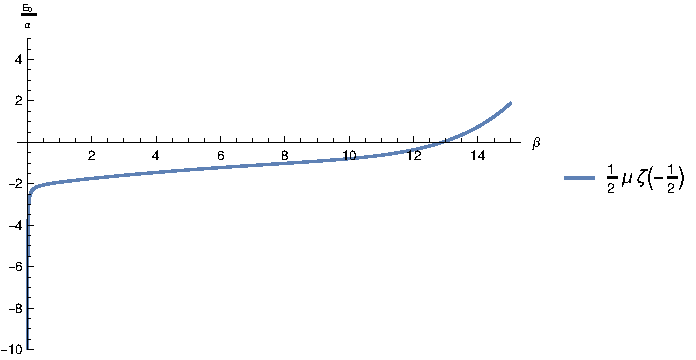
\includegraphics[height=1.0in]{Finita.pdf}
        \caption{Aquí se divide a ambos miembros de la ecuación \ref{eq.graficar} por $				\alpha$, de aquí se puede ver que la energía de vacío es siempre atractiva.}
        \label{fig.izquierda}
    \end{subfigure}%
    ~ 
    \begin{subfigure}[t]{0.5\textwidth}
        \centering
        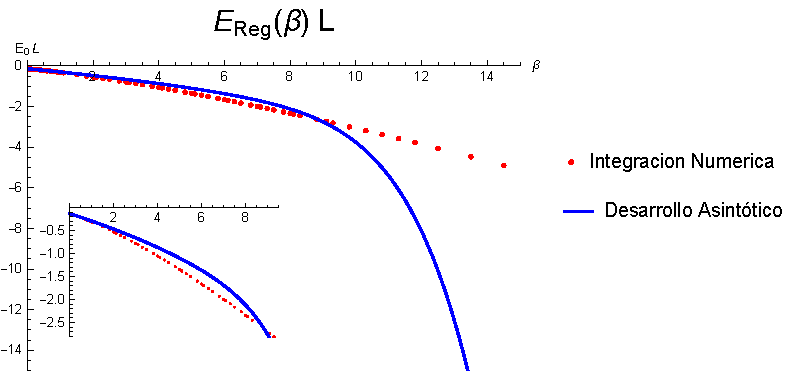
\includegraphics[height=1.0in]{exportar1.pdf}
        \caption{Aquí se multiplica a ambos lados \ref{eq.graficar} por $L$, ademas 				se puede apreciar en el inset que en el limite $\beta \rightarrow 0$ la energía 		tiende a $- \frac{1}{12}$}
        \label{fig.derecha}
    \end{subfigure}
    \caption{En esta imagen se muestran dos posibles adimensionalizaciones de la ecuación \ref{eq.graficar}, que representan la energía de vacío independiente de $\mu$ .}
\label{fig.finitas}
\end{figure*}

\begin{figure*}[t!]
    \centering
    \begin{subfigure}[t]{0.5\textwidth}
        \centering
        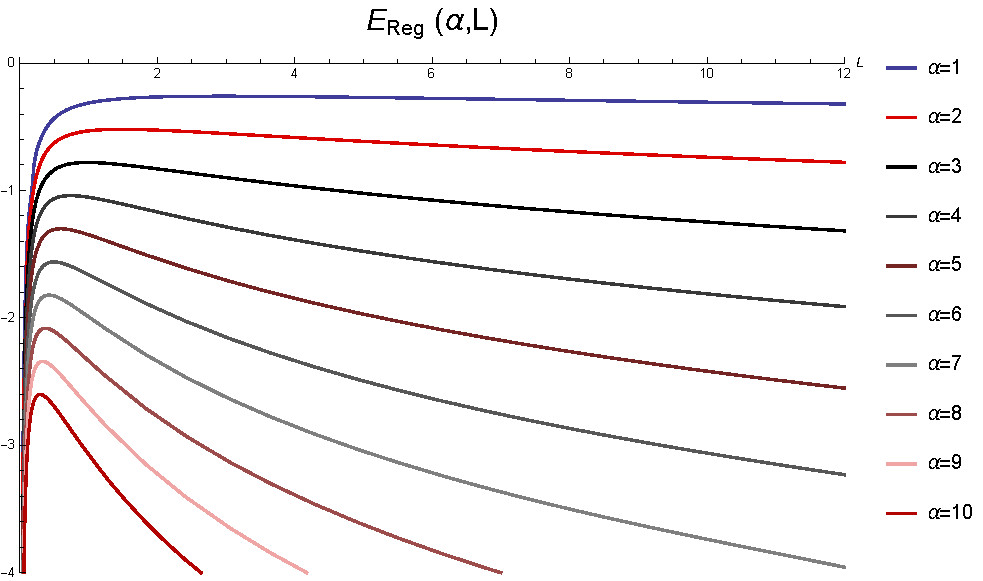
\includegraphics[height=1.45in]{Energias.pdf}
        \caption{}
%        \label{fig.izquierda}
    \end{subfigure}%
    ~ 
    \begin{subfigure}[t]{0.5\textwidth}
        \centering
        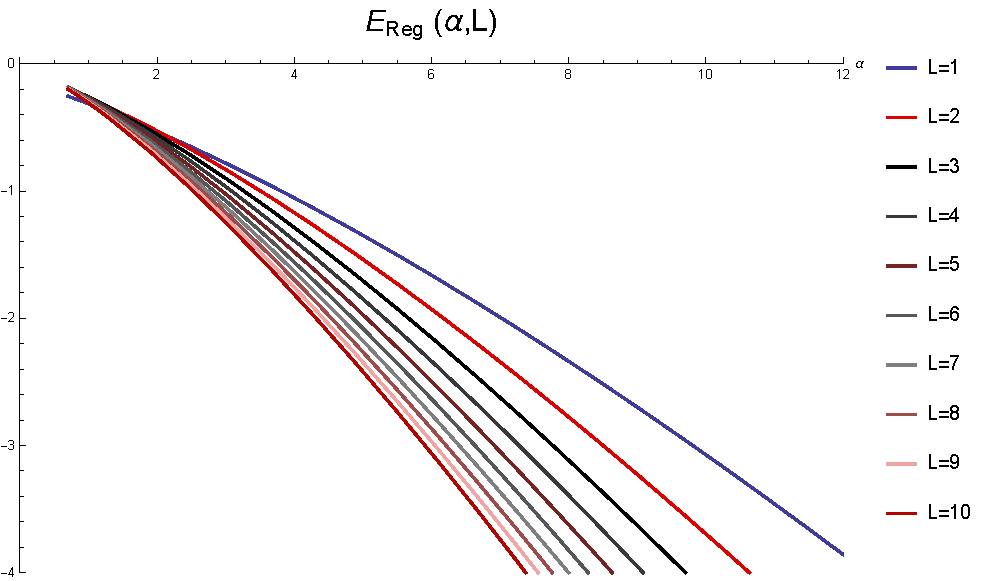
\includegraphics[height=1.45in]{Ls.pdf}
        \caption{}
%        \label{fig.derecha}
    \end{subfigure}
    \caption{En esta imagen se muestra la energía de Casimir $E _0$ para distintos valores de $\alpha$ en función de la longitud del intervalo $L$, puede verse que a medida que incrementa $\alpha$ la energía de vacío posee un máximo local mas abrupto.}
\label{fig:vacios}
\end{figure*}

\subsection{Parte finita de la energía de vacío la venganza }

En la sección \ref{sec.complejo} se mostró que la función $\zeta (s)$ puede representarse mediante una integral en el plano complejo, junto con posibles caminos que permiten calcular esta integral en la figura \ref{fig:contorno}. En los dos capítulos anteriores \ref{cap.sencillos}  y \ref{cap.singular} se utilizó el contorno \ref{fig.derecha} para obtener la estructura de polos, en este capítulo se utilizará el contorno \ref{fig.derecha.derecha} para obtener tanto los polos como su parte finita en $s = - \frac{1}{2}$.

Al igual que en los capítulos \ref{cap.sencillos}  y \ref{cap.singular} la energía de vacío queda expresada como la integral
\begin{equation}
	\zeta (s) = 
	\frac{1}{2 \pi i} \int _{\mathcal{C}} 
						\left( \frac{\lambda}{\mu} \right) ^{-2s}
						\partial _ \lambda 
						\log F _1 ^{1} 
						\left( 1+\frac{ \alpha}{2 \lambda i },
							2,2 i \lambda x 
							\right)												
						d \lambda
	\, .
\end{equation}
Utilizando las variables adimensionales $\beta = \alpha L$ y  $\tau = \lambda L$ la ecuación anterior puede reescribirse de la forma
\begin{align}
\label{eq.ultima.int}
	\zeta (s) =& 
	\frac{\left(L \mu \right)^{2s}}{2 \pi i} \int _{\mathcal{C}} 
	f (\tau , \beta) \tau ^{-2s} d \tau 
\, ,
\end{align}
donde $f( \tau, \beta)$ está dada por
\begin{align}
f(\tau, \beta) =& 	
i
\frac{
		\left(1 + \frac{ \beta}{2 i \tau} \right) 
		F _1 ^1 
			\left( 2 + \frac{ \beta}{2 i \tau} ,3 ,2 i \tau \right)
		+ \left( \frac{\beta				
				}
				{2 \tau ^2 } 
				\right)
				( F _{1} ^1 ) ^{(1,0,0)}
				\left( 1 + \frac{\beta}{2 i \tau} ,2 ,2 i \tau
						\right)
		}
		{F _1 ^1 \left( 1 + \frac{\beta}{2 i \tau},2,2 i \tau \right)} 
\, .		
\nonumber
\end{align}
Utilizando el camino de integración \ref{fig.derecha.derecha}, la integral \ref{eq.ultima.int} puede reescribirse como suma de cuatro integrales
\begin{align*}
\zeta (s) = 
- \frac{L ^{2s}}{2 \pi } 
\Bigg(&	  e ^{- i \pi s} \int _0 ^{C _0}
			f (i t,\beta )
			t ^{-2s}  dt 
		+ e ^{- i \pi s} \int _{C _0} ^{\infty}
			f (i t,\beta )
			t ^{-2s}  dt \\
		+&e ^{i \pi s} \int _{0} ^{C _0} 
			f (-i t,\beta )
			t ^{-2s}  dt 
		+ e ^{i \pi s} \int _{C _0} ^{\infty}
			f (-i t,\beta )
			t ^{-2s}  dt 
	\Bigg)
\, ,
\end{align*}
Donde la primer y tercer integral pueden calcularse de manera numérica en $s= -\frac{1}{2}$ dado que allí son convergentes. La segunda y la cuarta contienen el término divergente de $\zeta \left(- \frac{1}{2} \right)$ calculado en la ecuación (\ref{eq.result.zeta.c}), para calcular la parte finita de estas integrales se utiliza el desarrollo \ref{eq.aprox} obteniendo
\[ 
f   ( i t ,\beta )=
\begin{cases} 
	  f _{+} ( t, \beta) = 
	  i  \left(
			\frac{1}{t} - \frac{\beta}{2 t ^2 } + \frac{\beta}{2 t^2}
			\log (2 t) + \frac{\beta \gamma}{2 t^2} 
			\right) + O (t ^{-3})
	  & t > 0 \\
	  f _{-} ( t, \beta) =
      i  \left(
			- \frac{1}{t} + \frac{\beta}{2 t ^2 } - \frac{\beta}{2 t^2}
			\log (2 t) - \frac{\beta \gamma}{2 t^2} +2
			\right) + O (t ^{-3})
      & t < 0
   \end{cases}   
\]
Utilizando este desarrollo las ultimas dos integrales pueden expresarse
\begin{align}
\nonumber
	\int _{C _0} ^{\infty}
			f (i t,\beta )
			t ^{-2s}  dt &= 
	\int _{C _0} ^{\infty}
		\left(
			f (it, \beta) - f _{+} (t, \beta )			
				\right) t ^{-2s} dt 
	\\ &+ 
\nonumber
	\int _{C _0} ^{\infty}
			f _{+} ( t, \beta)
			 t ^{-2s} dt  \\
\nonumber
	\int _{C _0} ^{\infty}
			f (-i t,\beta )
			t ^{-2s}  dt &= 
	\int _{C _0} ^{\infty}
		\left(
			f (-it, \beta) - f _{-} (t, \beta )			
				\right) t ^{-2s} dt 
	\\ &+ 
\nonumber
	\int _{C _0} ^{\infty}
			f _{-} ( t, \beta)
			 t ^{-2s} dt
\end{align}
Donde las términos de arriba pueden integrarse numéricamente en $s=-1/2$ dado que son convergentes. 

Las contribuciones divergentes están dadas por
\begin{align}
\label{arriba}
&
	\int _{C _0} ^{\infty}
			f _{+} (t, \beta )			
			 t ^{-2s} dt =  
	O \left( s + \frac{1}{2} \right)
\\[5pt]
\nonumber			
&+
	i \left(- C _0 
		    - \frac{\beta \log C_0 (\gamma + \log 2 - 1 ) 
		    		}{2} 
		    - \frac{\beta \log ^2 C _0}{4}
		    + \frac{\beta ( \gamma + \log 2 -1 )}{4 (s + 1/2)} 
		    + \frac{\beta}{8 (s + \frac{1}{2}) ^2}
					\right)
\\[5pt]
\label{abajo}
&
	\int _{C _0} ^{\infty}
			f _{-} ( t, \beta)
			 t ^{-2s} dt =
	O \left(s + \frac{1}{2} \right)
\\[5pt]
\nonumber
&+
	i \left(C _0 
			- C _0 ^2
		    + \frac{\beta \log C_0 (\gamma + \log 2 - 1 ) 
		    		}{2} 
		    + \frac{\beta \log ^2 C _0}{4}
		    - \frac{\beta ( \gamma + \log 2 -1 )}{4 (s + 1/2)} 
		    - \frac{\beta}{8 (s + \frac{1}{2}) ^2}
					\right)
\end{align}
%%Esta integral no se si ponerla completa o no...
\begin{comment}
\begin{align}
\nonumber
&
	\int _{C _0} ^{\infty}
			f _{+} (t, \beta )			
			 t ^{-2s} dt =  
				i \left(
						\frac{C _0 ^{-2s}}{2s} +
						\frac{ \beta C _0 ^{-2s-1}}
							 {4} \left(
										\frac{\gamma  + \log 2 C_0 -1}
										{s + 1/2}
										+ \frac{1}{2 (s + 1/2) ^2}
										\right)
						\right)
\\[5pt]
\nonumber			
&=
	i \left(- C _0 
		    - \frac{\beta ( 2 \gamma + \log 4 C _0 -2 ) \log C_0
		    		}{4} 
		    + \frac{\beta ( \gamma + \log 2 -1 )}{4 (s + 1/2)} 
		    + \frac{\beta}{8 (s + \frac{1}{2}) ^2}
					\right)
\\
&
	+ O \left( s + \frac{1}{2} \right)
\\[5pt]
\nonumber
&
	\int _{C _0} ^{\infty}
			f _{-} ( t, \beta)
			 t ^{-2s} dt  \\
& 
=
\nonumber
				i \left(
						\frac{C _0 ^{-2s+1} }{s - \frac{1}{2}}
						- \frac{C _0 ^{-2s}}{2s} 
						- \frac{ \beta C _0 ^{-2s-1}}
							 {4} \left(
										\frac{\gamma  + \log 2 C_0 -1}
										{s + 1/2}
										+ \frac{1}{2 (s + 1/2) ^2}
										\right)
						\right)
\\[5pt]
\nonumber
&=
	i \left(
			- C _0 ^2 
			+ C _0 
		    + \frac{\beta ( 2 \gamma + \log 4 C _0 -2 ) \log C_0
		    		}{4} 
		    - \frac{\beta ( \gamma + \log 2 -1 )}{4 (s + 1/2)} 
		    - \frac{\beta}{8 (s + \frac{1}{2}) ^2}
					\right)
\\
	& + O \left(s + \frac{1}{2} \right)
\end{align}
\end{comment}
Se obtiene entonces para $\zeta \left( - \frac{1}{2} \right)$
\begin{eqnarray}
\zeta \left( - \frac{1}{2} \right) &=& 
- \frac{i}{2 \pi L \mu} 
\Bigg(	  
		 \int _{C _0} ^{\infty}
			\left(
					f (i t,\beta )
					- f (-i t,\beta )
					- f _{+} (t) 
					+ f _{-} (t)
					\right)
			t   dt   \nonumber
\\ \nonumber
&&\hskip 1.5cm +
		 \int _{- C _0} ^{C _0}
			f (i t,\beta )
			t   dt 	
	\Bigg)
\\ \nonumber
&&
	- \frac{\beta \log ^2 C _0}{4 \pi L \mu}
	- \frac{\beta \log C _0 (\gamma + \log 2 -1 )}{2 \pi L \mu} 
	- \frac{16 C_0 - 8 C _0 ^2 + \pi ^2 \beta}{16 \pi L \mu}
\\ \nonumber
&&
	+\frac{\beta \log ^2 (L \mu )}{4 \pi L \mu} 
	+ \frac{\beta \log  (L \mu) (\gamma + \log 2 -1)}{2 \pi L \mu}
\\ 
&&	+ \frac{\beta}
		 {8 \pi L \mu  \left( s + \frac{1}{2} \right) ^2} +
	\frac{\beta (\gamma + \log (2 L \mu) -1 ) }
		 {4 \pi L \mu  \left( s + \frac{1}{2} 														 \right)} 
\, .
\end{eqnarray}
Donde en la última linea se están los polos calculados en REF, y en la penultima linea la dependencia con la escala $\log (L \mu)$














